
\section{I2C Bus Overview}
\begin{frame}{I2C Bus Overview}
    \begin{itemize}
        \item Designed by Philips in 1982 (physical level).
        \item SMBUS created by Intel in 1995; adds timing, protocols, and operation modes to I2C.
        \item Uses two bidirectional open-drain lines (which need Pull-up's resistors):
        \begin{itemize}
            \item Serial Data Line (SDA)
            \item Serial Clock Line (SCL)
        \end{itemize}
        \item Typical voltages: +5 V or +3.3 V.
        \item Defines basic types of messages (using the digital signals):
        \begin{itemize}
            \item Master writes data to a slave.
            \item Master reads data from a slave.
            \item Combined messages with at least two reads/writes.
            \item[\hspace{1em}] 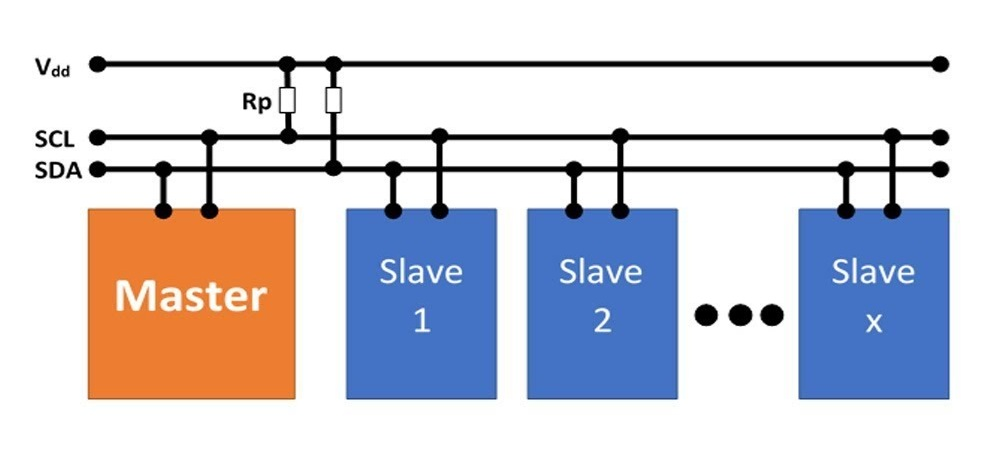
\includegraphics[width=0.5\textwidth]{trainingmaterials/i2c/i2cbasic.jpg}
        \end{itemize}
    \end{itemize}
\end{frame}

\begin{frame}{I2C Overview II}
    \begin{itemize}
        \item Any given slave will only respond to certain messages, as specified in its product documentation
        \item In practice, most slaves adopt request/response control models, where one or more bytes following a write command are treated as a command or address.
        \item Appropriate for peripherals where simplicity and low manufacturing cost are more important than speed.
        \item Common applications:
        \begin{itemize}
            \item Reading configuration data from memory sticks (e.g., DDR SDRAM).
            \item Accessing NVRAM chips for user settings.
            \item Controlling OLED/LCD displays.
            \item Reading real-time clocks and hardware monitors.
            \item Turning power supply on/off for system components.
        \end{itemize}
    \end{itemize}
\end{frame}

\begin{frame}{I2C Protocol}
    \begin{itemize}
        \item Communications are always started by the master.
        \item Messages consist of:
        \begin{itemize}
            \item Start condition: SDA falling edge with SCL high.
            \item Slave address: 7/10 bits.
            \item Read/Write bit: Read=1, Write=0.
            \item Acknowledge (Ack/Nack): Slave acknowledgment.
            \item Data bytes written by master or slave.
            \item Stop condition: SDA rising edge on SCL high.
        \end{itemize}
    \end{itemize}
\end{frame}

\begin{frame}{I2C Protocol II: Signal messaging}
    \begin{itemize}
        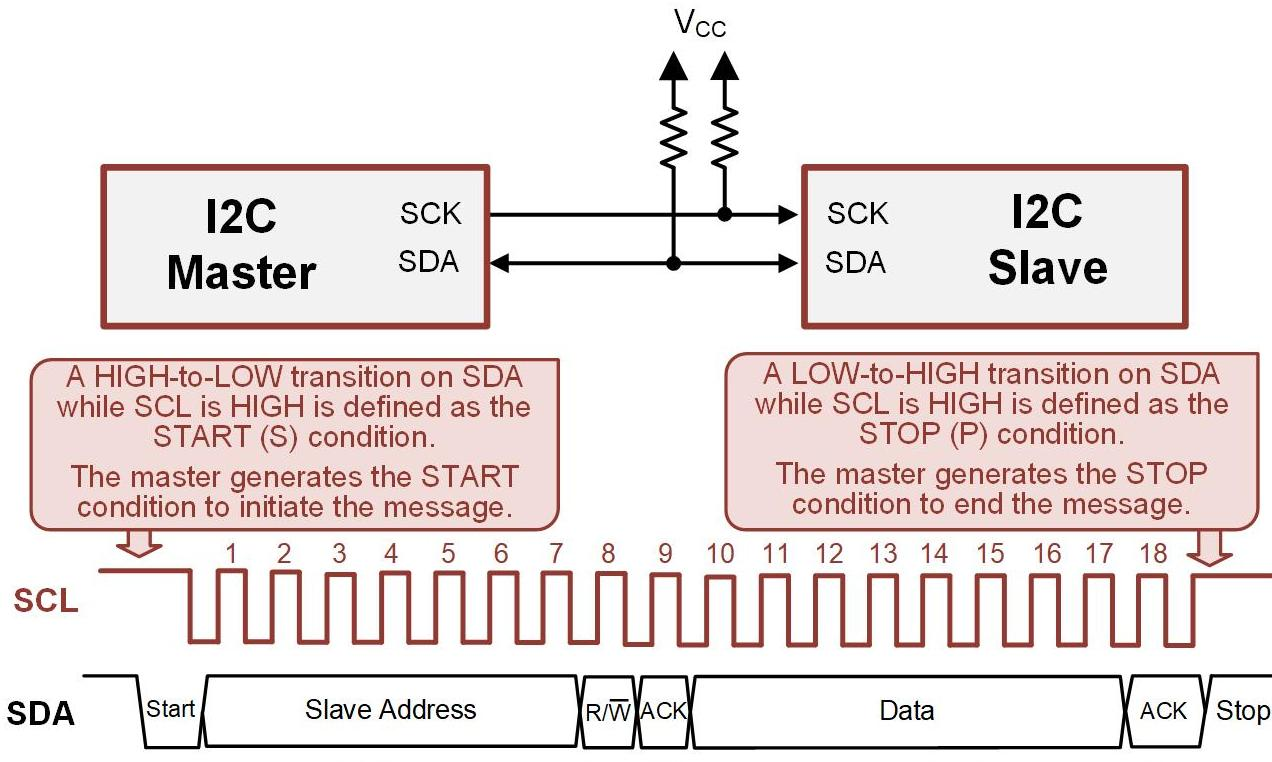
\includegraphics[width=\textwidth]{trainingmaterials/i2c/i2c-signals.jpg}
    \end{itemize}
\end{frame}

\begin{frame}{I2C Protocol III: Logic analyzer}
    \begin{itemize}
        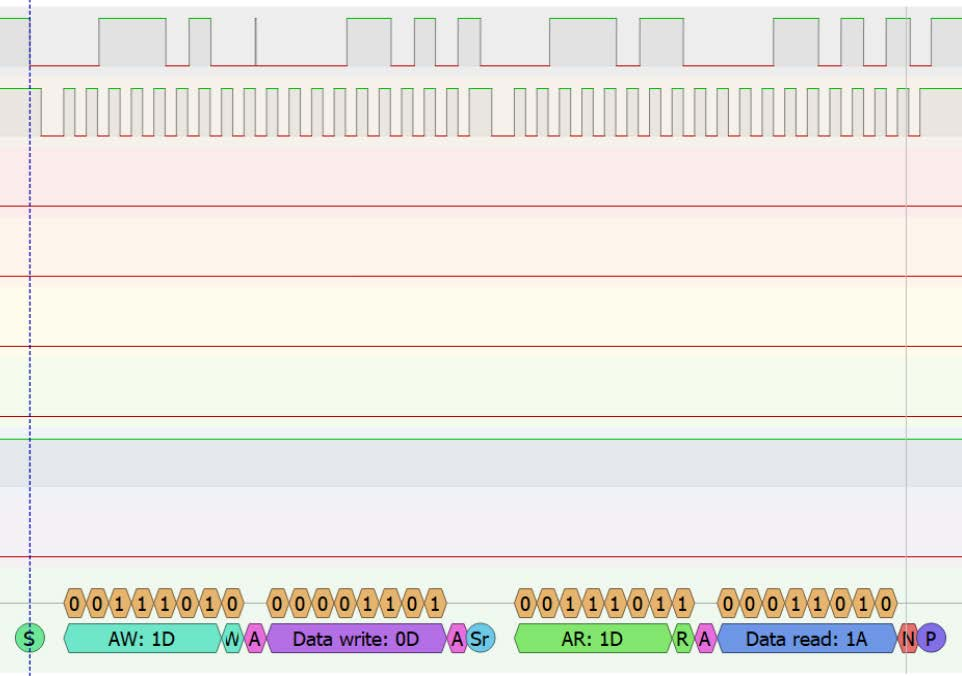
\includegraphics[width=0.9\textwidth]{trainingmaterials/i2c/i2c-signal-logic-analyzer.jpg}
    \end{itemize}
\end{frame}

\section{I2C in Linux}
\begin{frame}{Using I2C Devices in Linux}
    \begin{itemize}
        \item Devices represented as files under \texttt{/dev}.
        \item Examples of devices:
        \begin{itemize}
            \item Console/GUI Terminals
            \item RAM Blocks
            \item GPIO ports
            \item Serial line
            \item SD Card, USB Drives
            \item I2C interface
        \end{itemize}
        \item Enable I2C with \texttt{raspi-config}.
    \end{itemize}
\end{frame}

\begin{frame}[fragile]{I2C Program Example}
    \textbf{Code Snippet:}
    \begin{minted}[fontsize=\small, bgcolor=blue!5]{c}
//include files omitted
//Structs needed for I2C messages
struct i2c_rdwr_ioctl_data packets;
struct i2c_msg messages[2]; //Set size depending on number of messages in one transaction
char write_bytes[w_len];
char read_bytes[r_len];

int main(){
    char i2cFile[15];
    int addr = 0x5d; 
    sprintf(i2cFile, "/dev/i2c-%d", dev);
    int fd = open(i2cFile, O_RDWR); 
    ioctl(fd, I2C_SLAVE, addr);
    .............

    \end{minted}

\end{frame}

\begin{frame}[fragile]{I2C Program Example}
    \textbf{Code Snippet:}
    \begin{minted}[fontsize=\small, bgcolor=blue!5]{c}
//Prepare message(s)


    //Example of Write message
    messages[0].addr  = addr;
    messages[0].flags = 0; //means write
    messages[0].len   = w_len;
    messages[0].buf   = write_bytes; //Pointer to the data bytes to be written 
    // Example of Read message
    messages[1].addr  = addr;
    messages[1].flags = I2C_M_RD;
    messages[1].len   = r_len; 
    messages[1].buf   = read_bytes; //Pointer for reading the data
    //Build packet list
    packets.msgs      = messages;
    packets.nmsgs     = 2;

    \end{minted}

\end{frame}

\begin{frame}[fragile]{I2C Program Example}
    \textbf{Code Snippet:}
    \begin{minted}[fontsize=\small, bgcolor=blue!5]{c}
//Send message(s)
ioctl(handle->fd, I2C_RDWR, &packets);

//Parse data received in read_bytes
Value = read_bytes[0] * …
.
.
.


//Close file descriptor before exiting program
close (fd);

    \end{minted}

\end{frame}


\section{MPU-6050 Overview}
\begin{frame}{MPU-6050 Features}
    \begin{itemize}
        \item \textbf{Accelerometer:}
        \begin{itemize}
            \item Digital-output triple-axis accelerometer.
            \item Programmable full-scale range: ±2g, ±4g, ±8g, ±16g.
            \item Integrated 16-bit ADCs for simultaneous sampling.
        \end{itemize}
        \item \textbf{Gyroscope:}
        \begin{itemize}
            \item Digital-output X-, Y-, and Z-axis angular rate sensors.
            \item Full-scale range: ±250, ±500, ±1000, ±2000°/sec.
            \item Integrated 16-bit ADCs for simultaneous sampling.
        \end{itemize}
    \end{itemize}
\end{frame}

\section{Project Structure}
\begin{frame}{Structure for Project 1}
    \textbf{System Initialization:}
    \begin{itemize}
        \item Read input parameters.
        \item Display welcome message.
        \item Open sensor handler and configure it.
    \end{itemize}
    \textbf{System Operation:}
    \begin{itemize}
        \item Activate sensor.
        \item Loop through:
        \begin{itemize}
            \item Sample sensor data.
            \item Transform data to engineering units.
            \item Control sample frequency.
            \item Detect end condition.
        \end{itemize}
    \end{itemize}
    \textbf{System Closure:}
    \begin{itemize}
        \item Free allocated resources.
    \end{itemize}
\end{frame}


